\documentclass[a4paper,11pt]{article}

% ---------------------------------------------------------
% ENCODING / LINGUA
% ---------------------------------------------------------
\usepackage[T1]{fontenc}
\usepackage[utf8]{inputenc}
\usepackage[english]{babel}
\usepackage{csquotes}

% ---------------------------------------------------------
% LAYOUT PAGINA
% ---------------------------------------------------------
\usepackage[a4paper,left=2.5cm,right=2.5cm,top=2.5cm,bottom=2.5cm]{geometry}

% ---------------------------------------------------------
% PACCHETTI GENERALI
% ---------------------------------------------------------
\usepackage{enumitem}
\usepackage{fancyhdr}
\usepackage{multicol}
\usepackage{textcomp}
\usepackage{eurosym}

\usepackage{graphicx}
\usepackage{subcaption}
\usepackage{float}        % per [H]
\usepackage{booktabs}
\usepackage{indentfirst}
\usepackage{multirow}
\usepackage{makecell}
\renewcommand\theadfont{\bfseries}

\usepackage{xcolor}
\usepackage[version=4]{mhchem} % evita warning mhchem
\usepackage{siunitx}
\sisetup{group-separator={\,}, group-minimum-digits=4}

% ---------------------------------------------------------
% LISTINGS (CODICE)
% ---------------------------------------------------------
\usepackage{listings}
\lstset{
    basicstyle=\ttfamily\small,
    breaklines=true,
    numbers=left,
    numberstyle=\tiny,
    frame=single,
    keywordstyle=\color{blue},
    commentstyle=\color{gray},
    stringstyle=\color{orange},
    language=Matlab
}

% ---------------------------------------------------------
% MATEMATICA
% ---------------------------------------------------------
\usepackage{amsmath,amsfonts,amssymb,mathrsfs,bm,dsfont,mathtools,bigints,cancel}
\renewcommand{\vec}[1]{\mathbf{#1}}
\newcommand{\mat}[1]{\bm{\mathsf{#1}}}

% ---------------------------------------------------------
% STRUTTURA E TITOLI
% ---------------------------------------------------------
\usepackage[explicit]{titlesec}

\numberwithin{subsubsection}{subsection}
\numberwithin{subsection}{section}
\renewcommand{\thetable}{\Roman{table}}

% Colors
\definecolor{navy}{RGB}{0,0,128}
\definecolor{teal}{RGB}{0,128,128}
\definecolor{crimson}{RGB}{220,20,60}
\definecolor{olive}{RGB}{128,128,0} % <-- aggiunta

% Formatting sections
\titleformat{\section}
  {\Large\bfseries\color{navy}}
  {\thesection}
  {0.8em}
  {#1}
  [{\titlerule[0.8pt]}]

\titleformat{\subsection}
  {\large\bfseries\color{teal}}
  {\thesubsection}
  {0.8em}
  {#1}

\titleformat{\subsubsection}
  {\bfseries\color{olive}}
  {\thesubsubsection}
  {0.8em}
  {#1}

% ---------------------------------------------------------
% COMANDI PERSONALIZZATI
% ---------------------------------------------------------
\setlength{\parindent}{0pt}

\newcommand{\PRLsep}{\noindent\makebox[\linewidth]{\resizebox{0.45\linewidth}{1pt}{$\bullet$}}}
\newcommand{\figref}[1]{Figure~\ref{#1}}
\newcommand{\tabref}[1]{Table~\ref{#1}}
\newcommand{\secref}[1]{Section~\ref{#1}}
\newcommand{\chapref}[1]{Chapter~\ref{#1}}
\newcommand{\eqrefx}[1]{Equation~(\ref{#1})}

\usepackage{newunicodechar}
\newunicodechar{ʻ}{ʻ}

% ---------------------------------------------------------
% BIBLIOGRAFIA (BIBLATEX + BIBER)
% ---------------------------------------------------------
\usepackage[style=ieee,backend=biber]{biblatex}
\addbibresource{Bibliography.bib}

% ---------------------------------------------------------
% HYPERREF (VERSO LA FINE)
% ---------------------------------------------------------
\usepackage[
  pdftex,
  pdfauthor={Francesco Qualizza},
  pdftitle={Report Station BlackOut - Safety Analysis},
  hidelinks,
  colorlinks=true,
  linkcolor=blue,
  citecolor=blue,
  urlcolor=blue,
  linktoc=page
]{hyperref}

\date{\today}
% ---------------------------------------------------------
% HEADER/FOOTER
% ---------------------------------------------------------
\pagestyle{fancy}
\fancyhf{}
\lhead{\small \textsc{Regulation and Safety}}
\rhead{\small \textsc{Station BlackOut - Safety Analysis}}
\cfoot{\thepage}
\renewcommand{\headrulewidth}{0.5pt}

% ---------------------------------------------------------
% DOCUMENT
% ---------------------------------------------------------
\begin{document}

% ----------------- TITLE PAGE -----------------
\begin{titlepage}
\begin{flushleft}
 \vspace*{-1.5cm}\hspace*{-1.5cm}
\includegraphics[scale=0.4]{Images/logo-ETSEIB-UPC.png}
\end{flushleft}

\centering
\vspace*{4cm}

{\Huge \bfseries \textsc{Regulation and Safety}}\\[1cm]
{\huge\emph{Station BlackOut - Safety Analysis}}\\[1.5cm]
{\LARGE Filippo Dalmonego}\\[0.3cm]
{\LARGE Tyler Ewald}\\[0.3cm]
{\LARGE Riccardo Fasano}\\[0.3cm]
{\LARGE Francesco Qualizza}\\[0.3cm]
\vspace{4cm}
{\Large Supervisor:}\\[0.3cm]
{\Large Jordi Freixa}\\[0.3cm]
\vspace{2cm}
{\large \today}\\[0.3cm]
\end{titlepage}

% ----------------- TOC -----------------
\clearpage
\pagenumbering{roman}

\setcounter{tocdepth}{3}
\tableofcontents

\clearpage
\pagenumbering{arabic}

% ----------------- INTRO (non numerata ma nel ToC) -----------------
\section*{Introduction}
\addcontentsline{toc}{section}{Introduction}
The aim of this report is to present the first part of the Station Black-Out (SBO) project developed with RELAP5 as a system code. The main purpose of this first delivery is to study the reference model before any new safety-system design is introduced. In particular, the work is divided in two tasks: first, the verification of the steady-state conditions of the plant model and second the analysis of the SBO base case transient. The steady-state analysis is used to check that the model starts from physically consistent and stable operating conditions. The main thermal-hydraulic parameters are compared with the target values provided in the project statement, and their time evolution is checked in order to confirm that the initial condition is sufficiently stable for the transient calculations. After the steady-state verification, the SBO base case is analyzed. This case represents the reference accident scenario and is used as the starting point for the following parts of the project. The objective is to understand the sequence of events, the system response and the main thermal-hydraulic trends during the transient.

The reference plant selected for this analysis is the Zion Nuclear Power Station (United States), which was decommisioned in 1998. Although the real plant originally had four primary loops, the RELAP model used in this project is simplified into two equivalent loops only. One loop represents the broken loop and keeps the dimensions of a single loop, while the other represents the intact side and groups the remaining three loops into one single equivalent loop. 

\figref{fig:ZionNPP_Nodalization} shows the nodalization used in order to represent in the best way possible the Zion nuclear power plant.

\begin{figure}[H]
    \centering
    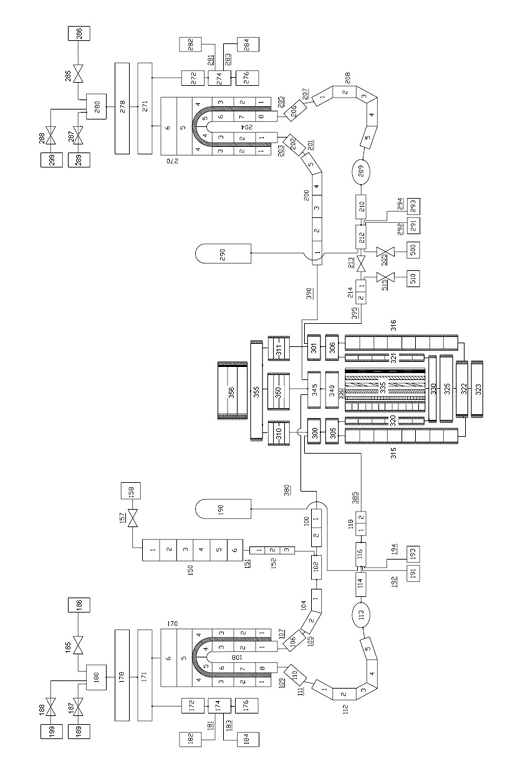
\includegraphics[width=0.85\textwidth]{Images/Nodalization of the Zion NPP.png}
    \caption{RELAP5 nodalization of the Zion Nuclear Power Plant model.}
    \label{fig:ZionNPP_Nodalization}
\end{figure}


\section{Steady State Analysis}
Before starting the accident analysis, it is necessary to verify that the model is in a stable and realistic initial condition.  
A correct steady state is important because the transient results strongly depend on the quality of the initial condition.
The steady-state run is checked by comparing the calculated values with the reference values and by observing the time evolution of the main parameters.  
If the variables remain approximately constant and the deviations from the target values are acceptable, the initial condition can be considered suitable for the transient simulation.
 



\begin{table}[H]
\centering
\caption{Reference values for steady-state verification.}
\label{tab:Targetvalues}
\begin{tabular}{l l l}
\toprule
\multicolumn{1}{c}{\textbf{Parameter}} & \textbf{Reference value} & \textbf{RELAP5 result} \\
\midrule
Power (MW) & 3250 & \\
Primary pressure in the hot leg (MPa) & 15.5 & \\
Secondary pressure (MPa) & 6.7 & \\
Pressurizer level (m) & 8.8 & \\
Broken SG downcomer level (m) & 12.2 & \\
Intact SG downcomer level (m) & 12.2 & \\
Core outlet temperature (K) & 603 & \\
Core inlet temperature (K) & 571 & \\
Broken Main FW flow (kg/s) & 459 & \\
Intact Main FW flow (kg/s) & 1325 & \\
Intact loop flow (kg/s) & 12865 & \\
Broken loop flow (kg/s) & 4351 & \\
\bottomrule
\end{tabular}
\end{table}

\tabref{tab:Targetvalues} shows the main variables that must be checked in the steady-state calculation.  
The last column is intentionally left empty for the simulation results, so that it can be completed later.


The steady-state calculation shows that the main plant variables are close to the reference values; small deviations may appear because of nodalization choices, control-system settings, and numerical approximations.  
However, the overall agreement is sufficient to accept the initial condition for the SBO transient analysis.

\section{Base Case Analysis}

After the steady-state verification, the SBO base case is studied. The Station Black-Out is assumed to begin at $t=0$ s with aggravated conditions. 
Under these conditions, every system that depends on electrical power is considered unavailable. 
As a result, the reactor coolant pumps trip, the control rods are inserted, and other relevant functions, such as the cooling of the pump seals, are lost. 
The general assumptions that are common to all the considered accident sequences are summarized in \tabref{tab:SBO_events} below.

\begin{table}[H]
\centering
\caption{Main events to be included in the SBO base case description.}
\label{tab:SBO_events}
\begin{tabular}{p{4cm} p{9cm}}
\toprule
\textbf{Event / action} & \textbf{Short description} \\
\midrule
SBO initiation & Loss of off-site and on-site AC power according to project assumptions \\
Reactor scram & Automatic shutdown following the transient logic \\
RCP trip & Reactor coolant pumps stop after loss of power \\
FW / AFW behavior & Feedwater and auxiliary feedwater response according to the base-case logic \\
Pressurizer systems & Heater and control-system behavior during SBO \\
Safety injection unavailability & HPSI and LPSI unavailable during the transient \\
Steam line / relief actions & Valve actions according to the project assumptions \\
Additional operator actions & To be completed based on the adopted base-case procedure \\
\bottomrule
\end{tabular}
\end{table}

\section{Preliminary Conclusions}

From the first analyses, the system code RELAP5 can be used as the model basis for the next stages of the project. The steady-state calculation is first checked against the target values, and the SBO base case is then used to observe the main thermal-hydraulic response of the plant under blackout conditions.

At this stage, the report is intended as a structured first draft. The final discussion will be completed after adding the detailed numerical results, the transient plots, and the comparison with the additional scenarios required in the following stages of the project.



\end{document}
